\chapter{Electronics Symbols}
\label{appendixSymbols}

\begin{center}
\begin{tabular}{M{0.1\linewidth} | M{0.12\linewidth} | m{0.6\linewidth}}
\textbf{Symbol} & \textbf{Component} & \textbf{Description} \\
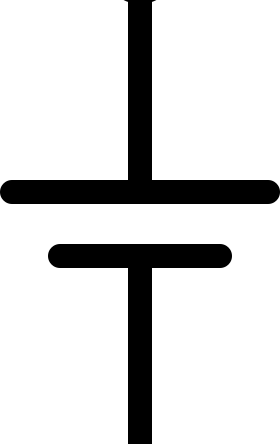
\includegraphics[scale=0.125]{BatterySymbol.png} & Battery & A battery is represented by a long line and a short line stacked on top of each other.  Sometimes, there are two sets of long and short lines.  The long line is the positive terminal and the short line is the negative terminal (which is usually used as the ground). \\ \hline
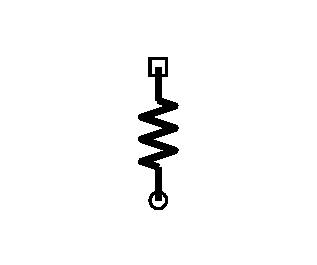
\includegraphics[scale=0.25]{ResistorSymbol.pdf} & Resistor & A resistor is represented by a sharp, wavy line with wires coming out of each side. \\ \hline
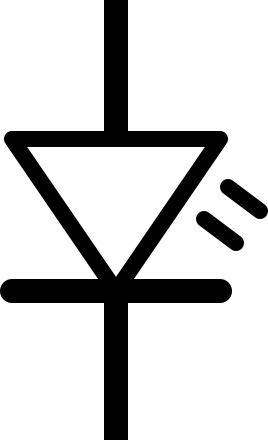
\includegraphics[scale=0.125]{LEDSymbol.png} & LED & An LED is represented by an arrow with a line across it, indicating that current can flow from positive to negative in the direction of the arrow, but it is blocked going the other way.  The LED symbol also has two short lines coming out of it, representing the fact that it emits light. \\
\end{tabular}
\end{center}

